\PassOptionsToPackage{table,xcdraw}{xcolor}

\documentclass[sigconf,review,anonymous]{acmart}
%\acmConference[ESEC/FSE 2021]{The 29th ACM Joint European Software Engineering Conference and Symposium on the Foundations of Software Engineering}{23 - 27 August, 2021}{Athens, Greece}

\acmConference[ICSE 2022]{The 44th International Conference on Software Engineering}{May 21–29, 2022}{Pittsburgh, PA, USA}

%\documentclass[sigconf,review, anonymous]{acmart}
%\documentclass[sigconf]{acmart}

\usepackage{booktabs}   %% For formal tables:
                        %% http://ctan.org/pkg/booktabs
\usepackage{subcaption} %% For complex figures with subfigures/subcaptions
                        %% http://ctan.org/pkg/subcaption
\usepackage{array}
\usepackage{amsmath,amsfonts}
\usepackage{algorithm}
\usepackage[noend]{algpseudocode}
%\usepackage{algorithmic}
\usepackage{graphicx}
\usepackage{textcomp}
\usepackage{float} 
\usepackage{listings}
\usepackage{xspace}
\usepackage{multirow}
\usepackage{amsthm}
\newtheorem{definition}{Definition}
\usepackage{balance}

\usepackage[skins]{tcolorbox}

\usepackage{xcolor,pifont}
\newcommand*\colourcheck[1]{%
	\expandafter\newcommand\csname #1check\endcsname{\textcolor{#1}{\ding{52}}}%
}
\colourcheck{blue}
\colourcheck{green}
\colourcheck{red}

\newtcolorbox{myframe}[2][]{%
  enhanced,colback=white,colframe=black,coltitle=black,
  sharp corners,
  toprule=1.0pt,
  rightrule=0.3pt,
  leftrule=0pt,
  bottomrule=0pt,
  fonttitle=\itshape\scshape\large,
  left=0pt,right=5pt,top=5pt,bottom=3pt,
  attach boxed title to top right={yshift=-0.3\baselineskip-0.4pt,xshift=-5mm},
  boxed title style={tile,size=minimal,left=0.2mm,right=0.5mm,
    colback=white,before upper=\strut},
  title=#2,#1
}

%\newcommand{\code}[1]{{\footnotesize\textsf{#1}}}

\newcommand{\tool}{\textsc{CDFix}\xspace}

\newtheorem{Definition}{Definition}
\newtheorem{Claim}{Claim}
\newtheorem{Lemma}{Lemma}
\newtheorem{Theorem}{Theorem}

\newcolumntype{L}[1]{>{\raggedright\arraybackslash}p{#1}}
\newtheorem{observation}{Observation}
\newtheorem{property}{Property}
\newcommand{\code}[1]{{\footnotesize\texttt{#1}}}
\usepackage{amsthm}
 \definecolor{dkgreen}{rgb}{0,0.6,0}
\definecolor{gray}{rgb}{0.5,0.5,0.5}
\definecolor{mauve}{rgb}{0.58,0,0.82}
\lstset{frame=tb,
  language=Java,
  aboveskip=3mm,
  belowskip=3mm,
  showstringspaces=false,
  columns=flexible,
  basicstyle={\small\ttfamily},
  numbers=left,
  numberstyle=\tiny\color{gray},
  keywordstyle=\color{blue},
  commentstyle=\color{dkgreen},
  stringstyle=\color{mauve},
  breaklines=true,
  breakatwhitespace=true,
  tabsize=4
}



\begin{document}

%\title[{\tool}: Deep Fault Localization with Code Coverage Representation Learning]{{\tool}: Deep Fault Localization with Code Coverage Representation Learning}

%\title[Deep Learning-Based Automated Program Repair:\\ Are We There Yet?]{Deep Learning-Based Automated Program Repair:\\ Are We There Yet?}

\title[Context-aware Dual-Task Learning for Automated Program Repair]{Context-aware Dual-Task Learning\\ for Automated Program Repair}

%%%---- AUTHORS BLOCK ------

%Yi Li:New Jersey Institute of Technology;Shaohua Wang:New Jersey
%Institute of Technology;Tien Nguyen:University of Texas at Dallas 

%\author{Yi Li}
%\affiliation{
%\institution{New Jersey Inst. of Technology, USA}
%}
%\email{yl622@njit.edu}
%\author{Shaohua Wang}
%\affiliation{
%\institution{New Jersey Inst. of Technology, USA}
%}
%\email{davidsw@njit.edu}
%\author{Tien N. Nguyen}
%\affiliation{
%\institution{University of Texas at Dallas, USA}
%}
%\email{tien.n.nguyen@utdallas.edu}


%\renewcommand{\shortauthors}{Li, Wang, and Nguyen}

\setcopyright{none}

\settopmatter{printacmref=false, printfolios=false}

\renewcommand\footnotetextcopyrightpermission[1]{} % removes footnote with conference information in first column


%(1) present information sorted in a way that a CNN can "see" patterns
%discriminating between faulty and non faulty statements more easily;

%(2) identify the actual crash statement to the network;

%(3) present more information to the deep neural network in the form of
%a summary of data dependences for each statement as well as source
%embedding; and

%(4) the suspiciousness of a statement is seen taking into account
%relationships to other statement, as opposed to a statement by itself”



%\input{sections/abstract}
\begin{abstract}
Abstract goes here ...
\end{abstract}


%\settopmatter{printacmref=true, printccs=true, printfolios=false}

%\begin{CCSXML}
%<ccs2012>
%<concept>
%<concept_id>10011007.10011006.10011073</concept_id>
%<concept_desc>Software and its engineering~Software maintenance tools</concept_desc>
%<concept_significance>500</concept_significance>
%</concept>
%</ccs2012>
%\end{CCSXML}

%\ccsdesc[500]{Software and its engineering~Software maintenance tools}

%\keywords{Deep Learning; Automated Program Repair; Context-based Code Transformation Learning}


\maketitle

\section{Introduction}

%Fixing software defects is one of the crucial maintenance
%activities. Thus,

%Detecting and fixing software defects is one of the most crucial
%activities in software development.
Researchers have developed the approaches to automate the
bug-fixing task. The approaches that help
developers automatically fix a software defect is
referred to as {\em automated program repair} (APR). The APR
approaches can be broadly classified in the following categories
based on their techniques:
%Researchers have proposed several approaches to help developers in
%automatically identifying and fixing the defects in programs. Such
%approaches are referred to as {\em automated program~repair}
%(APR). The APR approaches have been leveraging various techniques in
%the areas of
{\em search-based software engineering}, {\em software mining}, {\em
  machine learning (ML)}, and {\em deep learning (DL)}.

In search-based
approaches~\cite{LeGoues-icse12,le2011genprog,martinez2016astor,qi2014strength},
the buggy code is first mutated via certain operators to produce the
potential~solution space. A search strategy is designed to find
the fix in the solution space. Instead searching for a solution, the
software mining-based APR models learn the fixing patterns from
the prior bug
fixes~\cite{kim2013automatic,le2016history,liu2019avatar,tbar-issta19,nguyen2013semfix,
  icse10,ray-fse12}. Some mining-based approaches learn the patterns
from the source code~\cite{liu2019avatar,tbar-issta19} and others
learn them from prior bug-fixing
changes~\cite{wen2018context,Simfix,koyuncu2018fixminer}.  The fixing
patterns could be mined automatically from the repositories
or pre-defined via semi-automatic
techniques~\cite{le2016history,nguyen2013semfix,liu2019avatar,tbar-issta19}.

%Recent advances in
Machine learning (ML)
%enable several models to
has facilitated implicit learning from prior bug fixes to apply to repair
the current buggy
code~\cite{long2016automatic,long2017automatic,saha2017elixir}.
%They derive the candidate fixes and rank them according to their
%likelihoods
%researchers have leveraged deep learning (DL) to automatically derive
%the fixing changes to a given buggy code. Some
Some Deep Learning (DL)-based approaches learn the fix from prior {\em
  similar bug fixes and/or
  patterns}~\cite{gupta2017deepfix,white2019sorting,white2016deep}.
Other DL-based models treat APR as {\em machine translation} from a
buggy code to a correct one using transformers and other
models~\cite{chakrabortycodit,chen2018sequencer,hata2018learning,tufano2018empirical,see2017get}.
%Instead of treating APR as machine translation,
In addition, other DL-based approaches implicitly learn the {\em
  transformation rules} from a buggy code to a correct one accordingly
to the surrounding {\em context} of the
transformations~\cite{chen2018sequencer,icse20,cure-icse21,lutellier2020coconut}.
Those approaches show that {\em learning bug-fixing changes might be
  dependent on {\em code context}}, and they 
%For example, in C~code, if the preceding context contains \code{fopen}
%as in \code{FILE *fd = fopen (fname, ``rb'');}, the succeeding
%bug-fixing code is more likely to be \code{if (fd != null)} or
%\code{if (fd == null)}. However, if the preceding context contains
%\code{fread} as in \code{n} \code{=} \code{fread(buffer,1,size,fd);},
%the succeeding bug-fix is more likely to be \code{if (n} \code{!=}
%\code{size)} or \code{if (n} \code{==} \code{size)}, rather than a
%null check \code{if (n} \code{!=} \code{null)}.
%Those context-aware models
have achieved better APR
performance~\cite{icse20,lutellier2020coconut,cure-icse21}.

%For example, a {\em null check} is needed after a call to read data
%from a socket with \code{BufferedReader.readline} to make sure a
%successful data retrieval.
%tufano2019learning,chakrabortycodit}.

Despite recognizing the importance of contexts in learning the fixes,
the existing DL-based APR approaches over the time still have
limitations in {\em integrating context learning into code-change
  learning} in the APR process, leading to their ineffectiveness in
fixing context-dependent bugs.

First, the earlier DL-based approaches that learn from {\em bug-fixing
  patterns}~\cite{white2016deep,gupta2017deepfix} have focused on
similar code and/or code changes with {\em little or no consideration}
on whether those code or fixing patterns appear in certain surrounding
contexts. Second, in the same vein of taking too little or no context,
other DL-based APR approaches aim to learn {\em only the code changes}
for fixes, e.g., from a buggy subtree in an Abstract Syntax Tree (AST)
to the correct subtree \cite{chakrabortycodit,see2017get}. Despite
learning the code transformations for bug-fixing, taking no context
does not help a model learn the fixes that depend on a larger
surrounding code. In the third type of direction, some
approaches~\cite{hata2018learning,tufano2019learning,tufano2018empirical}
take too large context. They leveraged machine translation to take the
entire buggy method and translate it to the correct one, while the fix
might be only a small editing change to a single statement. Those
translation-based approaches do not distinguish clearly the boundary
of the fixing change (e.g., to a buggy statement) and the surrounding
context. Due to the mixture of fixing changes and context, those
translation models or transformers could pick the incorrect locations
for fixing, because they might not learn what fixing changes are
appropriate in some specific contexts~\cite{icse20}. Finally, the
recent DL-based
approaches~\cite{chen2018sequencer,cure-icse21,lutellier2020coconut,icse22}
extract contextual features to be fed into a single DL model to learn
to fix. However, they do not focus on context learning, despite that
{\em determining the correct context} is crucial to extract the right
features to help a model learn fix context-dependent bugs. Those
approaches do not help their models to correctly learn the contexts
given that the code transformations for bug-fixing are known and could
be used to train the models for context learning.


%\underline{First}, the DL-based APR approaches that learn from {\em
%  bug-fixing patterns}~\cite{white2016deep,gupta2017deepfix} have
%focused on similar code and/or code changes with {\em little or no
%  consideration} on whether those code or fixing patterns appear in
%certain surrounding contexts. \underline{Second}, some DL-based APR
%approaches aim to learn {\em only the code changes} for fixes, e.g.,
%from a buggy subtree in an Abstract Syntax Tree (AST) to the correct
%subtree \cite{chakrabortycodit,see2017get}. In this treatment, too
%little or no context might not help a model learn the fixes that
%depend on a larger surrounding code.

%\underline{Third}, other
%approaches~\cite{hata2018learning,tufano2019learning,tufano2018empirical}
%leveraged machine translation to take the entire buggy method and
%translate it to the correct one, while the fix might be only a small
%editing change to a single statement. Those translation-based
%approaches do not distinguish clearly the boundary of the fixing
%change (e.g., to a buggy statement) and the surrounding context.  Due
%to the mixture of fixing changes and context, those translation models
%or transformers could pick the incorrect locations for fixing, because
%they might not learn what fixing changes are appropriate in some
%specific contexts~\cite{icse20}. \underline{Fourth}, other DL-based
%approaches have separate representations for
%contexts~\cite{chen2018sequencer,cure-icse21,lutellier2020coconut}.
%They extract contextual features to be fed into a single DL model to
%learn to fix.

%\underline{Fifth}, dedicating a separate model for context learning
%has recently been shown to improve over the DL-based approaches with a
%single DL model~\cite{icse20}. In DLFix~\cite{icse20}, the first layer
%is a tree-based RNN model that learns the contexts of bug fixes (CCL)
%and its result is used as an additional weighting input for the second
%layer designed to learn the bug-fixing code transformations
%(CTL). However, the cascading from CCL $\rightarrow$ CTL
%creates a {\em confounding effect} from the inaccuracy of the learning
%of the context to that of the fix transformations.



%===============================================
%the DL-based APR approaches that leverage {\em machine translation or
%  transformers}~\cite{chakrabortycodit,hata2018learning,tufano2018empirical,see2017get}
%often take too little surrounding code as context to learn fixing
%changes or do not have a clear boundary of the fixing changes and the
%context. Let us elaborate this point. Some DL-based APR approaches aim
%to learn {\em only the code changes} for a fix, e.g., from one buggy
%subtree in an Abstract Syntax Tree (AST) or a buggy statement to the
%correct subtree or statement~\cite{chakrabortycodit}. In this
%treatment, too little context might not help a model learn the fixes
%that depend on a larger surrounding code. In contrast, other
%approaches~\cite{chen2018sequencer,hata2018learning} take the entire
%buggy method and translate it to the correct one, while the fix might
%be only a small editing change to a single statement. Those
%translation-based approaches {\em do not distinguish clearly the
%  boundary} of the fixing change (e.g., to a buggy statement) and the
%surrounding context (e.g., the preceding or succeeding code). Due to
%the mixture of fixing changes and context, those machine translation
%models or transformers might not learn what fixing changes are
%appropriate in specific contexts~\cite{icse20}.

%===============================================
%\underline{Third}, to address that issue, DLFix~\cite{icse20} makes a
%clear boundary of fixing changes and the surrounding context, and
%dedicates two layers for those two tasks. The first layer is a
%tree-based RNN model that learns the contexts of bug fixes and its
%result is used as an additional weighting input for the second layer
%designed to learn the bug-fixing code transformations. However, the
%cascading architecture in DLFix from the two layers create a
%confounding effect from the inaccuracy of the learning of the context
%to the learning of the bug-fixing code transformations.
%---------------------------------

%We conjecture that the two tasks of learning the code
%context and learning the bug-fixing code transformations are related
%and dependent on each other. {\bf Correct learning of contexts can
%  benefit the learning of code transformations and vice versa in
%  automated program repair}. For example, in C code, if the
%preceding code (i.e., part of the context) contains \code{fopen} as in
%\code{FILE *fd = fopen (fname, ``rb'');}, then the succeeding
%bug-fixing code is more likely to be \code{if (fd != null)} or
%\code{if (fd == null)}. However, if the preceding code contains
%\code{fread} as in \code{n = fread(buffer,1,size,fd);}, then the
%succeeding bug-fix is more likely to be \code{if (n != size)} or
%\code{if (n == size)}, rather than a null check \code{if (n !=
%  null)}. In contrast, if the bug fix is a
%change from \code{if (fd == null)} into \code{if (fd != null)}, then the
%preceding code more likely contains \code{fopen} than \code{fread}.
%Let us call such relation between two tasks as {\em duality}.

%{\bf Correct learning of contexts can benefit the learning of code
%  transformations and vice versa in automated program repair}

%Tien removed this para
%{\em Moreover, the equally important impact from CTL to CCL is not
%  considered. Such impact from the direction of CTL $\rightarrow$
%CCL, could help the model correctly learn the context, leading to
%better code-transformation learning for context-dependent bugs. In the
%previous example, if the bug fix is a change from \code{if (fd ==
%  null)} into \code{if (fd != null)}, the preceding context more
%likely contains \code{fopen(...)} than \code{fread(...)}.}

%Tien
In this work, we conjecture that to improve the learning of code
transformation for bug-fixing, we {\em dedicate a separate model for
  context learning}, rather than extract contextual features as in the
above approaches.
%
We introduce {\tool}, a context-aware, dual-task learning APR
approach, that improves APR via the {\em simultaneous tasks of context
  learning and code transformation learning}.  Context learning and
code-transformation learning are complementary to one another, leading
to better APR. For example, if the preceding context contains
\code{fopen} as in \code{FILE *fd = fopen (fname, ``rb'');}, the
succeeding bug-fixing code is likely \code{if (fd} \code{!=}
\code{null)} or \code{if (fd} \code{==} \code{null)}. However, if the
preceding context contains \code{fread} as in \code{n} \code{=}
\code{fread(buffer,1,size,fd);}, the succeeding fix is likely \code{if
  (n} \code{!=} \code{size)} or \code{if (n} \code{==} \code{size)},
rather than a null check \code{if (n} \code{!=} \code{null)}. In
contrast, because the {\em fixing code transformations are always known at
  training}, we leverage them for better context learning. For
example, if the fix is a change from \code{if (fd} \code{==}
\code{null)} into \code{if (fd} \code{!=} \code{null)}, the key
contextual features are more likely \code{fopen(...)} than
\code{fread(...)}.

\indent In {\tool}, we dedidate two models: CCL for context learning and CTL
for code-transformation learning. We use a model called~{\em
  cross-stitch unit}~\cite{misra2016cross} that connects CTL and
CCL. The sharing of representations between CCL and CTL is modeled
by~learning a linear combination of the input features from two
models. Cross-stitch unit helps regularize CCL and CTL by learning and
enforcing shared representations via combining feature maps. The
rationale for dual-task learning is to propagate the impact of CCL and
CTL and vice versa. {\em The impact from both directions helps both
  models learning better in its own task (better CCL leads to better
  CTL, which leads to better CCL, and so on), and finally leading to
  better generated patches}, which are derived from the CTL's output.

%Tien removed this
%Our idea is that to improve APR for context-dependent bugs, a model
%first needs to have better code-transformation learning for
%bug-fixing. It also needs better context learning, i.e., learning
%contextual features for a fix because incorrect context learning could
%make incorrect fixing for context-dependent bugs.
%%have {\em both better context learning} (learning the correct
%%contextual features for a bug fix) and {\em better code-transformation
%%  learning} (learning the correct modifications).
%For example, in C~code, if the preceding context contains \code{fopen}
%as in \code{FILE *fd = fopen (fname, ``rb'');}, the succeeding
%bug-fixing code is likely \code{if (fd} \code{!=} \code{null)} or
%\code{if (fd} \code{==} \code{null)}. However, if the preceding
%context contains \code{fread} as in \code{n} \code{=}
%\code{fread(buffer,1,size,fd);}, the succeeding fix is more likely
%\code{if (n} \code{!=} \code{size)} or \code{if (n} \code{==}
%\code{size)}, rather than a null check \code{if (n} \code{!=}
%\code{null)}. In contrast, if the fix is a change from \code{if (fd}
%\code{==} \code{null)} into \code{if (fd} \code{!=} \code{null)}, the
%key contextual features are more likely \code{fopen(...)} than
%\code{fread(...)}.

%Tien
%Talk about CTL is the main task

%{\em explicitly models the mutual impact of context learning and code
%  transformation learning in both directions}.
%We train the two models simultaneously with soft-sharing parameters
%to exploit the duality of CCL and CTL.
%
%Specifically, we use a model called {\em cross-stitch
%  unit}~\cite{misra2016cross} that connects CTL and CCL. The sharing
%of representations between CCL and CTL is modeled by learning a linear
%combination of the input features from two models.  Cross-stitch unit
%helps regularize both CCL and CTL by learning and enforcing shared
%representations by combining feature maps.
%This joint training enables the dual-task learning to propagate the
%impact of CCL and CTL and vice~versa.

%Tien removed this
%With dual-task learning, {\tool} has two key departure points to
%address the limitations of the existing DL-based~APR approaches: {\em
%  1) Conceptually, it models both directions of the mutual impacts of
%  CCL and CTL, leading to improve APR; 2) Architecturally, it
%  overcomes the confounding effect in the existing cascading
%  architecture} (Section~\ref{ccl:sec}.2.1). The internal structure of CCL
%and CTL, and their connections in {\tool} are also more advanced than
%DLFix (Section~\ref{eval-methodology:sec}).

For training, the input of the CCL model is the Abstract Syntax Tree
(AST) of a buggy method and that of the fixed one.
The input of the CTL model is the AST subtree of each of its buggy
statements, and that of the fixed statement. For
auto-fixing, a fault localization tool is used to identify the buggy
statement(s). The AST subtree of the buggy statement is fed into the
trained~CTL model~to produce the ranked candidate patches, which are
validated via test cases. We leverage a tree-oriented beam search for
efficiency.

%In {\tool}, for training, the input for the CCL model is the Abstract
%Syntax Tree (AST) of a buggy method and that of the fixed method, and
%the input of the CTL model is the AST subtree of each of its buggy
%statements, and that of the respective fixed statement. For
%auto-fixing, a buggy statement to be fixed is identified by a fault
%localization tool. Then, the AST subtree for the buggy statement is
%fed into the trained CTL model to produce the candidate patches. We
%design a novel tree-oriented beam search for efficiency. Finally, the
%candidate patches are ranked and validated via test cases.

We conducted experiments to compare {\tool} with the DL-based APR
models on Defects4J~\cite{defects4j} (395~bugs),
Bugs.jar~\cite{saha2018bugs} (1,158 bugs), and
BigFix~\cite{yioopsla19} (+4.9M methods and 1.8M buggy ones).
%
Our results show that CDFix can fix 4.7\%–-143\% and 5.7\%–-263\% more
bugs than the baseline models with only top-1 patches in Bugs.jar and
BigFix, respectively. It fixes 26.4\% and 27.7\% of the total bugs
that were missed by the best baseline. {\tool} auto-fixes 56 bugs,
i.e., 194.7\% (37 bugs), 40\% (16), 27.3\% (12), 16.7\% (8), 3.7\%
(2), 24.4\% (11), and 5.6\% (3) more bugs than
SequenceR~\cite{chen2018sequencer}, DLFix~\cite{icse20},
CoCoNuT~\cite{lutellier2020coconut}, CURE~\cite{cure-icse21},
CURE*~\cite{cure-icse21}, RewardRepair~\cite{monperrus-icse22}, and
DEAR~\cite{icse22} respectively.
%In Defects4J, {\tool} fixes 194.7\%, 40\%, 27.3\%, 16.7\%, and 3.7\%
%more bugs than the baselines: SequenceR~\cite{chen2018sequencer},
%DLFix~\cite{icse20}, CoCoNuT~\cite{lutellier2020coconut},
%CURE~\cite{cure-icse21}, and DEAR~\cite{icse22}, respectively.
{\tool} complements to the best baseline Recoder in Defects4J but
improves over it in Bugs.jar and BigFix. In Defects4J, since
generating only single-hunk patches, Recoder did not fix 16
multi-hunk/multi-statement bugs that {\tool} fixed.
% {\tool} fixed 8 more bugs than the next-best DL model,
%CURE~\cite{cure-icse21}.  Even with the cut-off setting in CURE
%(taking 10\% more time than {\tool}), CURE fixed 4 less bugs than
%{\tool}.  In Bugs.jar and BigFix, {\tool} fixes 12.1\% and 14.6\%
%more bugs than CURE~\cite{cure-icse21}, using only Top-1 patches,
%respectively. Moreover, {\tool} fixed 89 and 45 unique bugs that CURE
%missed, while {\tool} missed only 50 and 27 bugs that~were fixed by
%CURE in Bugs.jar and BigFix.


The contributions of this paper include:

%are listed as follows:

%{\bf A. DL for APR:} {\tool} is the first DL APR that generates
%comparable and complementary results with powerful pattern-based
%tools, as recently published DL-based APR can only fix very few bugs
%on Defects4J. {\tool} helps confirm that further research on building
%advanced DL to improve APR is promising and valuable.

%{\bf A. A Novel Dual-Task Learning DL-based APR Model:}

%1) Leveraging dual-task learning to propagate the {\bf mutual impacts}
%  in both directions of context and transformation learning.

1) {\tool}: uses dual-task learning to model mutual impacts of~context
learning and transformation learning, leading to better APR.

%2) Adapting/Modifying the cross-stitch unit for dual-task
%learning to work with AST representations in source code.

%2) A demonstration that mutual impacts of context learning
%and code transformation learning lead to better APR.

2) We show that dedicating a model for context learning improves APR
better than extracting contextual features.

%3) A novel {\bf tree-oriented beam search} for candidate generation.

%4) Dual-task architecture avoiding confounding inaccuracies.


%A context-aware APR approach that leverages dual learning {\em to
%  propagate the impact between context learning and bug-fixing code
%  transformation learning to improve APR}. We {\bf advance DL-based
%  APR} with {\bf explicit modeling of the impact of contexts} via {\bf
%  dual learning}.

%{\bf B. Dual Learning Technique for Context Learning.} to explicitly
%model the context and

%with the use of a dual learning scheme that exploits the duality of
%learning bug-fixing code transformations and learning code contexts to
%improve APR performance.

3) Empirical Results: 
%{\bf Advancing DL-based APR approaches with dual-task learning for CCL
%  and CTL}:
%Extensive experiments were performed to evaluate different aspects
%of {\tool} and comparison.
%We evaluated {\tool} against the DL-based models to show that it can
%fix more bugs than those approaches.
Experiments show {\tool}'s improvements over prior
DL-based APRs. Code and data are at~\cite{CDFix2022}.

%to evaluate {\tool} and show it improves
%APR performance over the existing DL-based approaches.

%{\bf B. Empirical Results:} (Code and data are published~\cite{CDFix2022}).
%{\bf Improving over all the DL-based APR approaches}: we evaluated
%{\tool} against the most recent DL-based models to show that it can
%auto-fix more bugs than those state-of-the-art approaches.

%{\tool} is able to detect 2.5 times more bugs than the best performing
%baseline.  {\tool} can fix 253 new bugs (out of 1158 in Bugs.jar) than
%all the other DL-based APR techniques combined.

%-------------------------------------------------------------

%{\bf 1. {\tool}: Novel DL-based fault localization approach} that
%derives the co-change fixing locations for a bug. Our idea is
%to treat such problem as a dual learning task with the joint training
%of the method-level and statement-level co-fixing learning models.

%{\bf 2. Novel graph-based representation learning with co-change
%  statements.} Our graph-based representation learning with GCN
%and the novel type of features in co-change statements enables
%the dual-task models learn derive co-change fixing locations.

%{\bf 3. Extensive empirical evaluation.} We evaluated {\tool} against
%the most recent FL models to show our model's better performance. Our
%replication package is available at~\cite{FixLocator2022}.

\section{Motivating Example}
\label{motiv:sec}

\subsection{An Example and Observations}

\begin{figure}[t]
	\centering
	\lstset{
		numbers=left,
		numberstyle= \tiny,
		keywordstyle= \color{blue!70},
		commentstyle= \color{red!50!green!50!blue!50},
		frame=shadowbox,
		rulesepcolor= \color{red!20!green!20!blue!20} ,
		xleftmargin=1.5em,xrightmargin=0em, aboveskip=1em,
		framexleftmargin=1.5em,
                numbersep= 5pt,
		language=Java,
    basicstyle=\scriptsize\ttfamily,
    numberstyle=\scriptsize\ttfamily,
    emphstyle=\bfseries,
                moredelim=**[is][\color{red}]{@}{@},
		escapeinside= {(*@}{@*)}
	}
	\begin{lstlisting}[]
    public LegendItemCollection getLegendItems() {
        LegendItemCollection result = new LegendItemCollection();
        if (this.plot == null) {
            return result;
        }
        int index = this.plot.getIndexOf(this);
        CategoryDataset dataset = this.plot.getDataset(index);
(*@{\color{red}{-\quad \quad \quad if (dataset != null) {}@*)
(*@{\color{cyan}{+\quad \quad \quad if (dataset == null) {}@*)
            return result;
        }
        int seriesCount = dataset.getRowCount();
        // update result ...
        return result;
    }
	\end{lstlisting}
        \vspace{-15pt}
        \caption{Mutual Impact between Context and Fixing Change}
        \vspace{-8pt}
        \label{fig:motiv}
\end{figure}

%       if (plot.getRowRenderingOrder().equals(SortOrder.ASCENDING)) {
%            for (int i = 0; i < seriesCount; i++) {
%                if (isSeriesVisibleInLegend(i)) {
%                    LegendItem item = getLegendItem(index, i);
%                    if (item != null) {
%                        result.add(item);
%                    }
%                }
%            }
%        }
%        else {
%            for (int i = seriesCount - 1; i >= 0; i--) {
%                if (isSeriesVisibleInLegend(i)) {
%                    LegendItem item = getLegendItem(index, i);
%                    if (item != null) {
%                        result.add(item);
%                    }
%                }
%            }
%        }

%Let us start with a real-world example to motivate our approach.
Figure~\ref{fig:motiv} shows a real bug from the project \code{Chart}
in the Defects4J dataset. The bug occurred at line 8 in which the
condition for stopping the updating process on the \code{result}
variable is incorrect (\code{if (dataset != null)}). The result is
returned only when the dataset (line 7) is empty. Thus, it was fixed
into \code{if (dataset == null)}.

\noindent {\bf Observation 1 [Fixing Change Depends on Context]}. As
seen, the bug-fixing change from line 8 to line 9 (\code{if (dataset
  != null)} $\rightarrow$ \code{if (dataset == null)}) depends on the
surrounding code context. On line 7, the dataset is retrieved via
\code{getDataset}. According to the logic of the program, the result
is returned when \code{dataset} is \code{null}.  Thus, the incorrect
checking was fixed into line 9. That is, that fix (rather than
\code{if (dataset == 0)}) makes sense in the context consisting of
the preceding code (\code{getDataset}, \code{getIndexOf},
\code{LegendItemCollection}, etc.), and the succeeding code
(\code{dataset.getRowCount}, \code{return result}, etc.).

\vspace{3pt}
\noindent {\bf Observation 2 [Context Depends on Fixing
    Change]}. Because of the change (\code{if (dataset != null)}
$\rightarrow$ \code{if (dataset == null)}), the key features in the
context could likely be \code{getDataset} and \code{getIndexOf},
rather than \code{this.plot == null} (line 3) or \code{return result;}
(line 4).

Despite successes, the state-of-the-art, DL-based approaches are
limited in integrating context learning and code-change learning.

\underline{First}, for the DL-based approaches that learn the fixes
from prior {\em similar bug fixes or
  patterns}~\cite{gupta2017deepfix,white2019sorting,white2016deep},
there might not be any fix similar to the one in
Figure~\ref{fig:motiv}. They focus on similar bug fixes with little or
no consideration on whether a fix appears in certain~context.

\underline{Second}, some other DL-based APR approaches focus {\em only
  on learning the changes} to fix an AST subtree or a
statement~\cite{chakrabortycodit,see2017get} without considering the
context. For this example, without examining the surrounding context,
e.g., the preceding code \code{getDataset} or the succeeding code
\code{getRowCount} or \code{return result}, such a model will
make the same change regardless of contexts.
%not likely learn to change line 8 into line 9.

%hata2018learning,tufano2019learning,tufano2018empirical

\underline{Third}, for the machine translation and transformer-based
APR
models~\cite{hata2018learning,tufano2019learning,tufano2018empirical},
the entire method in Figure~\ref{fig:motiv} is used as the input. {\em
  Without distinguishing the boundary of the context and the fixing
  changes}, such a model faces the noise, i.e., the code irrelevant to
the actual fix at lines 8--9. For example, the code at lines 2--5 on
the legends is not crucial for the fix regarding the dataset at line
9. Thus, such a model could identify the incorrect location to fix.

\underline{Fourth}, some other DL-based approaches have separate
representations for
contexts~\cite{chen2018sequencer,cure-icse21,lutellier2020coconut}.
SequenceR~\cite{chen2018sequencer},
CoCoNuT~\cite{lutellier2020coconut}, and CURE~\cite{cure-icse21}
extract features in the surrounding context (e.g., lines 2--7, lines
10--15) to be fed into a DL model to learn to fix.
%These approaches utilize only one DL model for learning the fixes
%using the features extracted from the contexts.

%\underline{Finally}, recent DL-based APR
%approaches~\cite{icse20,cure-icse21} have leveraged the context to
%help better fix a bug. They separately consider the surrounding code
%as the context (e.g., lines 2--7, lines 10--15).

\underline{Fifth}, a recent trend shows that
%DLFix~\cite{icse20} shows that
dedicating a separate model for context learning can achieve better
performance than using a single
model~\cite{icse20}. DLFix~\cite{icse20} has two models in which one
tree-based LSTM model learns the context and another one learns the
code transformation (e.g., from line 8 to line 9). It cascades the
first LSTM model to the second one in which the output of the model
for contexts is used as a weight for the transformation learning one.
Thus, DLFix~\cite{icse20} suffers two limitations: 1) it does not
capture well both directions of the mutual impact between two types of
learning (esp. from code-change learning to context learning), 2) it
creates confounding inaccuracies as explained.
%
%This cascading architecture creates a confounding effect from the
%inaccuracy of the learning of the context to the learning of the
%transformations.
In Section~\ref{sec:overlap}, we will present our study and examples
to illustrate this.

%those limitations of the existing DL-based APR approaches.

\subsection{Key Ideas}
\label{sec:key-idea}

%To address the above issue with the cascading architecture,



To advance DL-based APR, we {\bf {\em explicitly model both directions
    of the mutual impact between context learning and transformation
    learning}}. We design {\tool} that treats context learning and
transformation learning as a dual task between CCL and CTL.

%with code context learning model (CCL) and code transformation
%learning (CTL).

%{\tool} consists of two models. The first model, CCL, is dedicated to
%learn \underline{c}ode \underline{c}ontexts, and the second model,
%CTL, to learn bug-fixing \underline{c}ode \underline{t}ransformations.


%To avoid the confounding effect in a naive solution of detecting buggy
%methods first and then detecting buggy statements in those methods, we
%design an approach that treats detecting dependent CC fixing locations
%as a {\em dual learning} task between them. First, the {\em
%  method-level FL} model (\code{MethFL}) aims to learn the methods
%that need to be modified in the same fix. Second, the {\em
%  statement-level FL} model (\code{StmtFL}) aims to learn the
%co-fixing statements regardless of whether they are in the same or
%different methods.

Intuitively, the two models CCL and CTL are dependent on each
other. The learning of the contexts can benefit the learning of
bug-fixing code transformations and vice versa. We refer to this
relation as {\em duality}, which can provide useful constraints for
{\tool} to learn to fix {\em context-dependent bugs}. We conjecture
that the join training of the two models can improve the performance
of both, if we can achieve the shared representations. For example, in
Figure~\ref{fig:motiv}, if the context is observed as containing
\code{getDataset} at line 7, \code{getIndexOf} at line 6, and
\code{return result} at line 10, the likelihood of the fixing change
at line 8 becoming \code{(dataset == null)} is more than that of
\code{(dataset != 0)}. The rationale is that only if the retrieved
data is empty, the result is returned. On the other hand, if the
bug-fixing transformation is observed as \code{(dataset != null)}
becoming \code{(dataset == null)}, it is likely to have an assignment
\code{dataset = ...;} in the context preceding \code{(dataset !=
  null)}.  Therefore, in {\tool}, we joinly train CTL for context
learning and CCL for transformation learning with soft-sharing of
parameters to exploit their relation.

Specifically, {\bf {\em we have adapted/modified the cross-stitch
    unit \cite{misra2016cross} to work with AST representations}} to
connect CTL and CCL. The sharing of representations between them is
modeled by the learning a linear combination of the input features
from two models. Cross-stitch unit helps regularize both CCL and CTL
by learning and enforcing shared representations by combining feature
maps. This joint training {\em propagates the mutual impact} of
context learning and transformation learning. {\em The use of
  cross-stitch unit also helps avoid confounding inaccuracies} in the
cascading architecture.

%and vice versa, to improve APR performance.

\section{{\tool}: Approach Overview}
\label{overview:sec}

%{\tool} has two main processes: training and predicting.


\subsection{Training Process}

Figure~\ref{overview-training} shows the overview of our training
process. If a method has multiple buggy statements, we treat one buggy
statement and~its enclosing method at a time as a training
instance. The input of~this process is the source code of a buggy
method and one of its buggy statements, and the respective fixed
source code.  The output includes the trained tree-based CCL model and
the trained tree-based CTL model.
%
%code context learning model (CCL model to learn the surrounding code
%context) and the trained tree-based code transformation learning model
%(CTL model to learn the bug-fixing code transformations) with their
%parameters.
The training process has two main steps:

\begin{figure}[t]
	\centering
	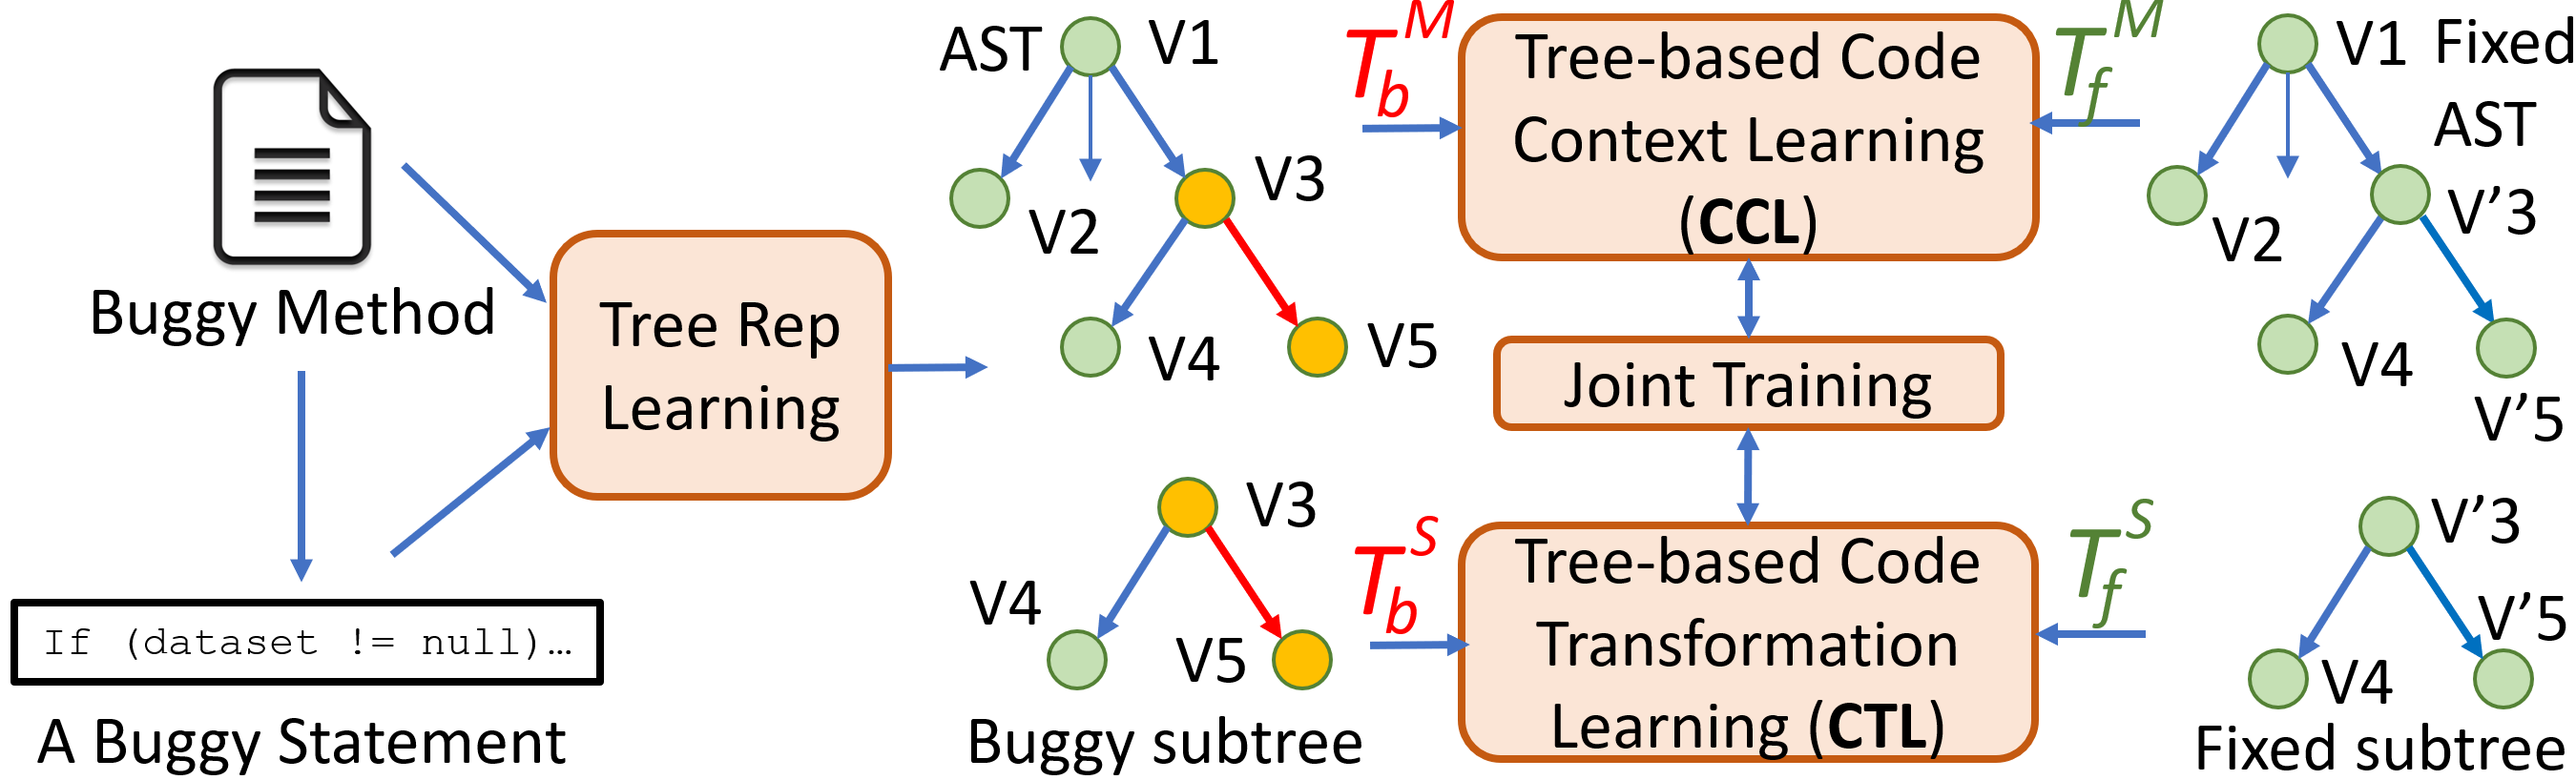
\includegraphics[width=3.4in]{graphs/new_overview-2.png}
        \vspace{-15pt}
	\caption{{\tool}: Training Process}
	\label{overview-training}
%	\vspace{-10pt}
\end{figure}

%\vspace{3pt}
\noindent {\bf Tree-based Representation Learning.} This step aims to
take the source code and to build the tree-based vector
representations (embeddings) to be the inputs of CCL and CTL. To
achieve that, the given method is parsed to obtain its AST
and the subtree for the buggy statement.
%we first parse the given source code to obtain the AST for the given
%method and the subtree for the buggy statement.
Then, the word embedding technique, GloVe~\cite{pennington2014glove},
is used to produce the vector for each node in the AST when we flatten
the AST into a sequence. The output of this step is the AST for the
method and the AST subtree for the buggy statement
in which each node is replaced by its embedding vector
(Figure~\ref{overview-training}).

\vspace{3pt}
\noindent {\bf Context-aware, Dual-Task Learning Automated Program
  Repair.}  The goal of this step is to train both the tree-based CCL
and the tree-based CTL in a joint-training manner. The entire AST
$T^{M}_b$ of the buggy method after vectorization (i.e., each node is
a vector) is used at the input layer of CCL for training. The AST of
the corresponding fixed method $T^{M}_f$ after vectorization is used
at the output layer of the CCL model. Similarly, the AST subtree
$T^{S}_b$ of the buggy statement after vectorization is used at the
input layer of CTL, and the subtree $T^{S}_f$ of the corresponding
fixed statement after vectorization is used at the output layer of
CTL. The CCL and CTL models are realized via attention-based
\code{seq2seq} models.
%Instead of cascading the two models CCL and CTL,
We use the {\em cross-stitch unit}~\cite{misra2016cross} to train CCL
and CTL simultaneously with soft-sharing the parameters to exploit
this duality. Joint training is aimed to learn the shared
representations between CCL amd CTL in terms of a linear combination
of the input features in both models. The output of this step includes
the trained CCL and CTL models.

\subsection{Prediction Process}



Figure~\ref{overview-fixing} illustrates the prediction process, i.e.,
the automated fixing process. A common usage of our tool is that
a developer could first use a fault localization tool
(FL) to detect the buggy statements that need to be fixed. Then, the
input for {\tool} is a buggy statement in the enclosing method.
%Another usage is that a developer can pinpoint the buggy statement and
%invoke {\tool} for an auto-fixing suggestion.
The fixing process shares the first step of Tree-based Representation
Learning with the training process. After that step, the vectorized
buggy AST subtree (each tree node is represented by a vector), is used
as the input of the {\em trained tree-based} CTL. The output of the
trained CTL model is the fixed AST subtree, which is converted back
into source code to form a candidate patch. We design a novel patch
generation that uses beam search over the AST structure and works in
accordance with the decoder as part of CTL in order to improve
efficiency. Finally, we adopt the patch validation process via test
cases as in DLFix~\cite{icse20}.

%the candidate patches are validated and output.

%We design a novel patch validation scheme that makes use of beam
%search for an efficient process. The final candidate patches are then
%produced.

\begin{figure}[t]
	\centering
	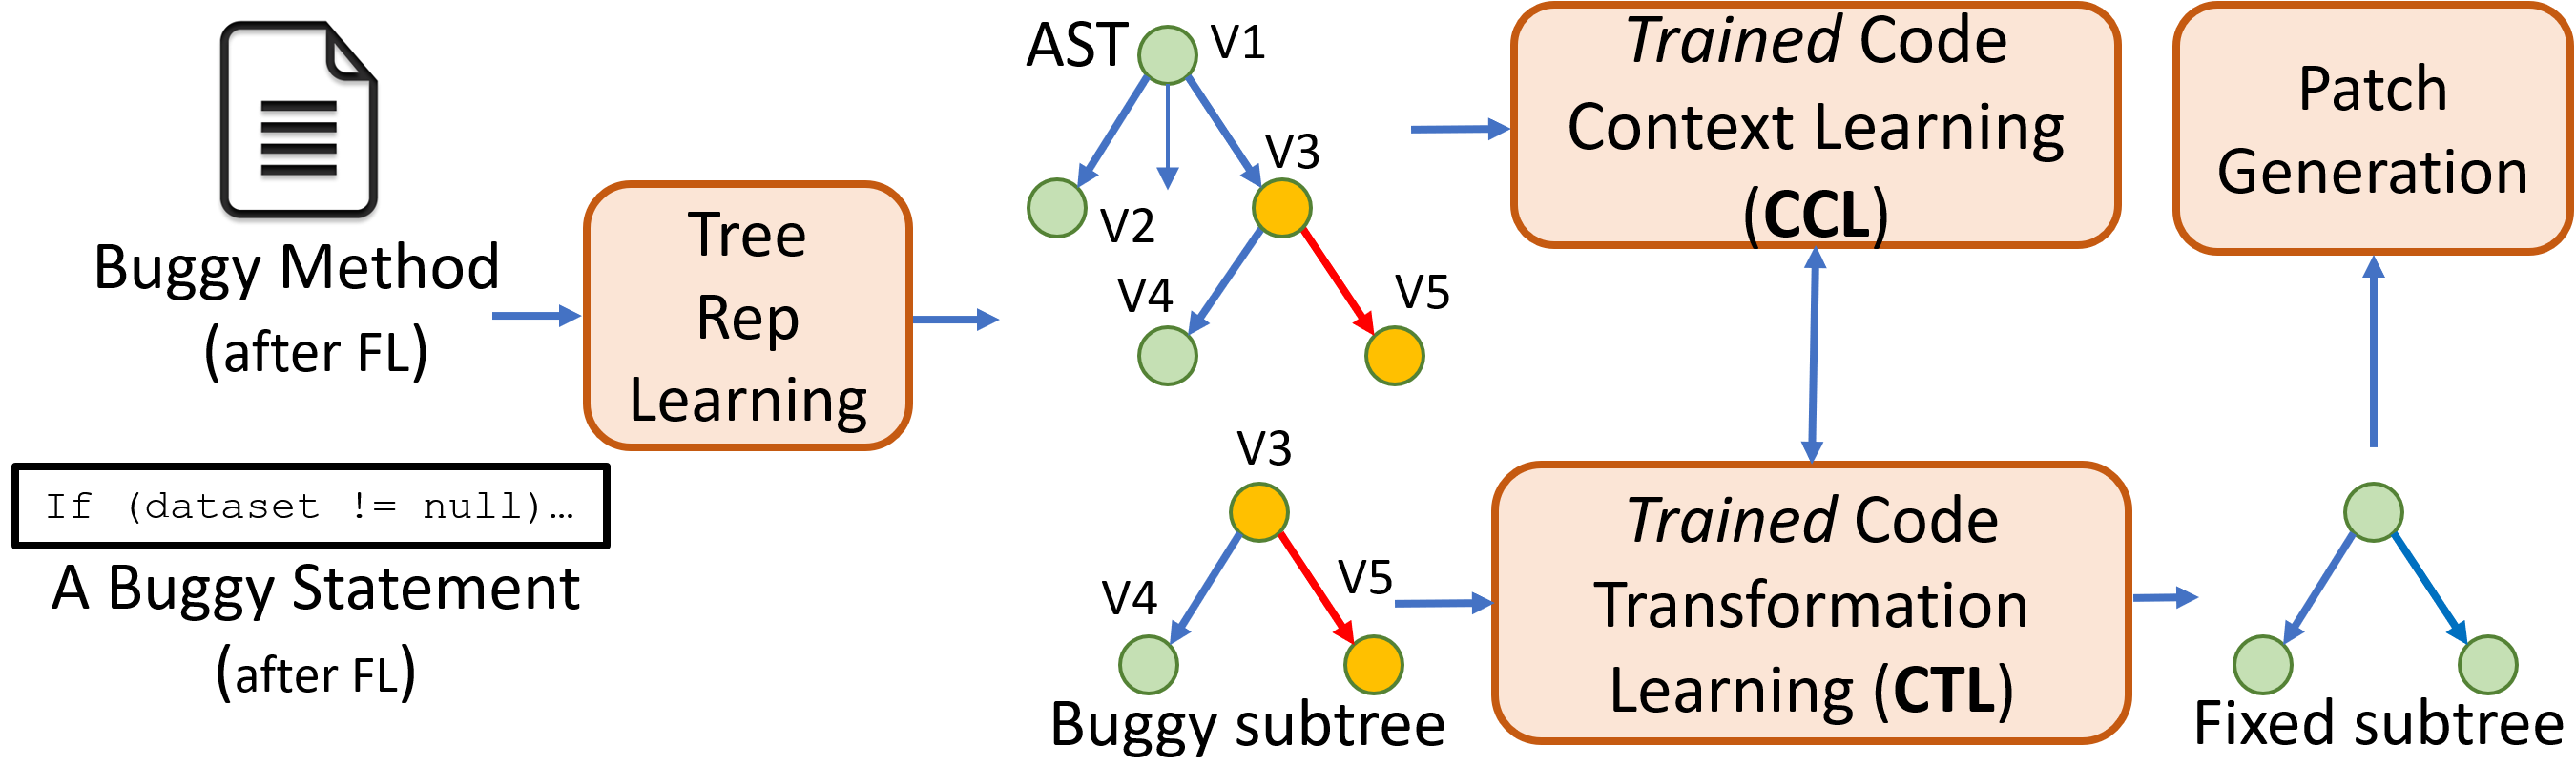
\includegraphics[width=3.4in]{graphs/overview-predict-2.png}
	\caption{{\tool}: Fixing Process}
        \vspace{-3pt}
	\label{overview-fixing}
\end{figure}

\section{Tree-based Representation Learning}

%\begin{figure}[t]
%	\centering
%	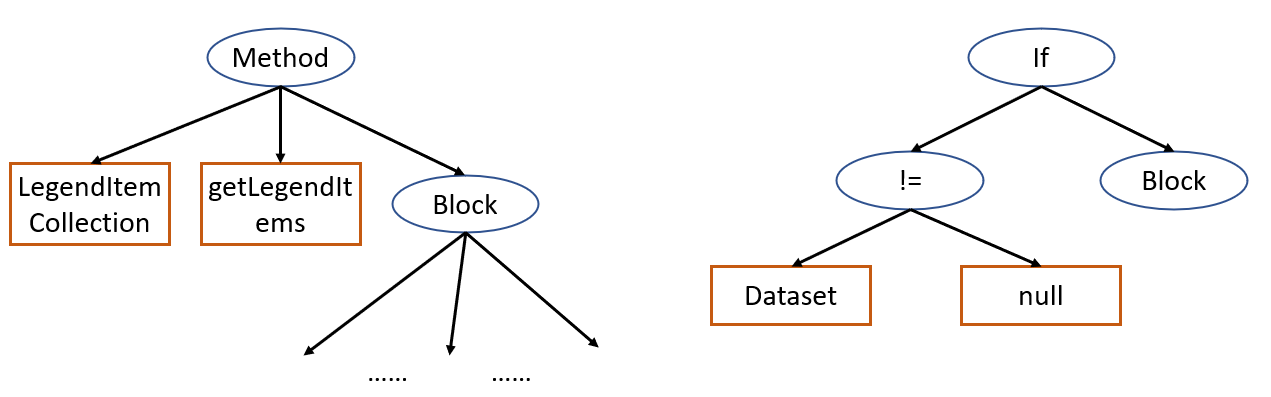
\includegraphics[width=3.2in]{graphs/tree_extraction.png}
%	\caption{Abstract Syntax Tree Extraction Example}
%	\label{tree-extraction}
%\end{figure}

%The goal of this step is to take the source code under study and to
%build the vector representations (embeddings).

This step aims to build the embeddings for the given source code.

\begin{figure}[t]
	\centering
	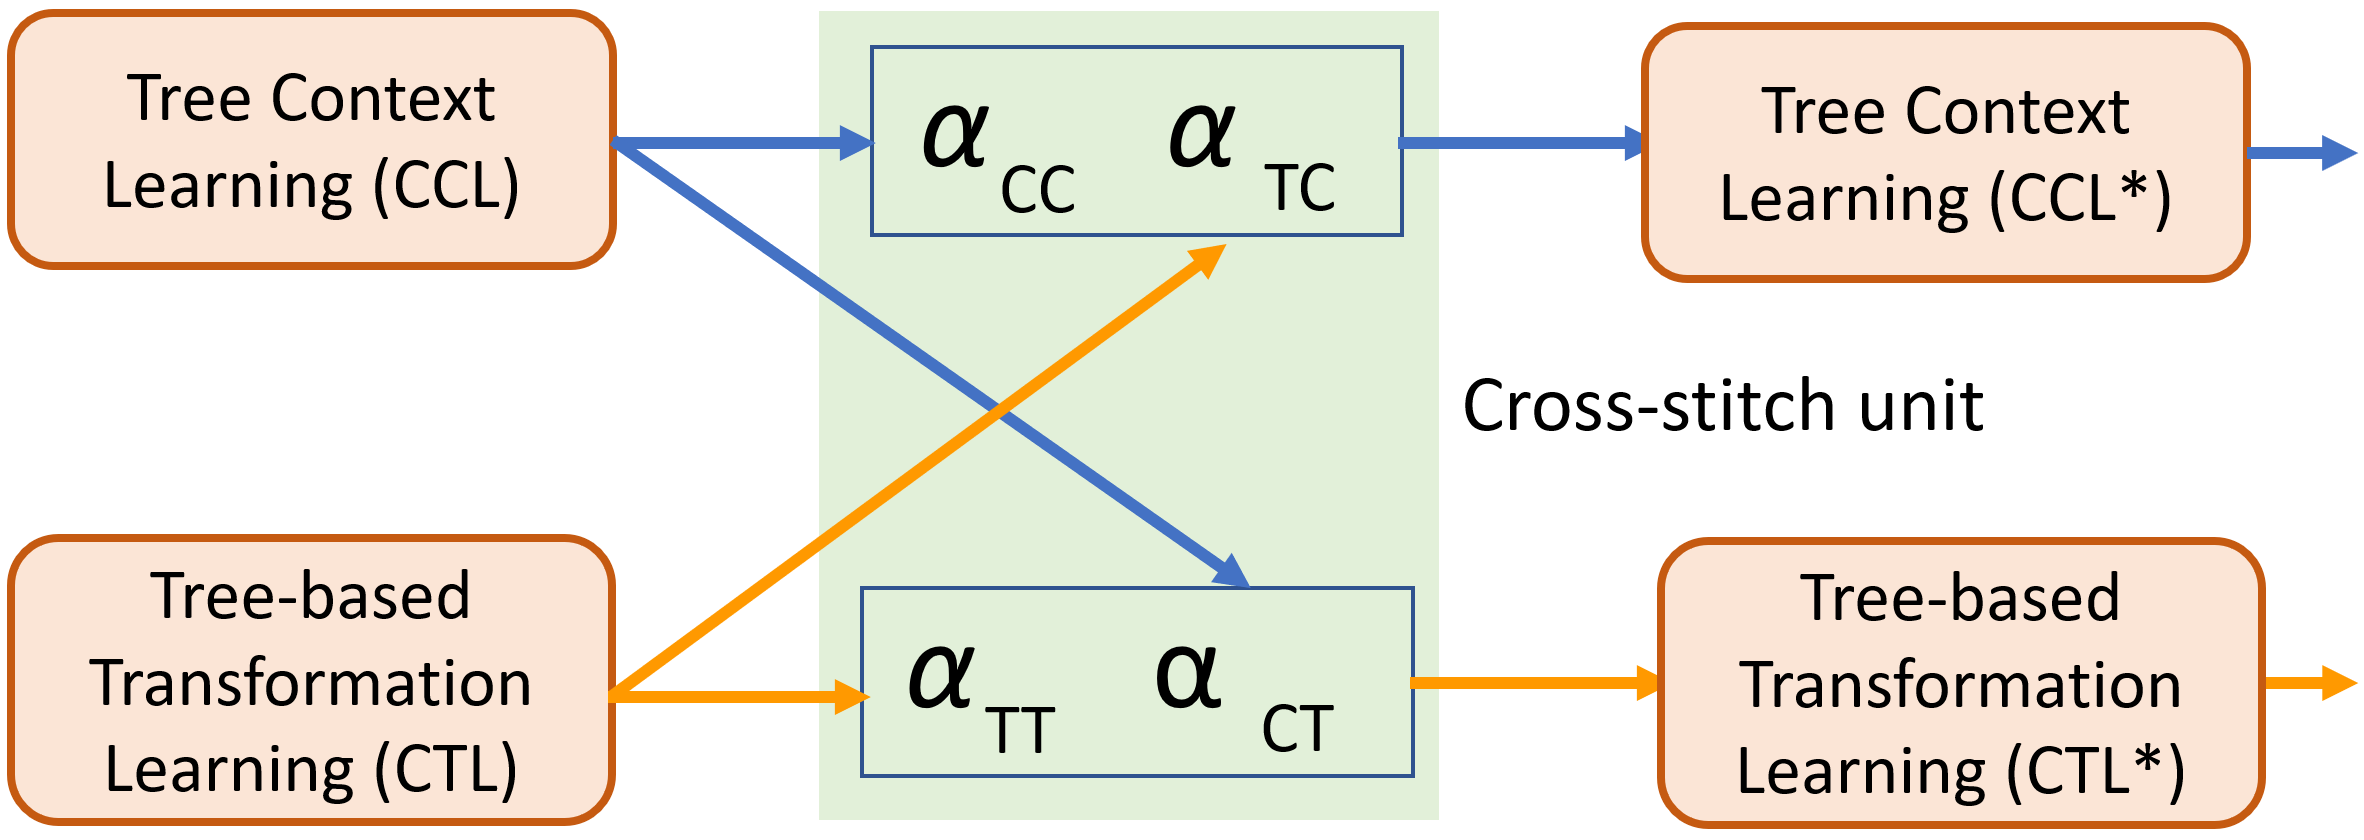
\includegraphics[width=2.8in]{graphs/cross-stitch}
        \vspace{-6pt}
	\caption{Cross-Stitch Unit for Joint Training~\cite{misra2016cross}}
	\label{fig:cross-stitch}
\end{figure}


%\subsection{AST Building and Pairing of Subtrees}

For a buggy method $M$, we parse the code to build the AST for
$M$. We identify the subtree $T_s$ for each buggy
statement $s$. If there are multiple buggy statements~in $M$, we
generate multiple AST subtrees, and use a buggy~statement
together with $M$ as a training instance for CCL and CTL.
%to train the context learning and code transformation models.
We use the tree differencing tool, CPatMiner~\cite{nguyen2019graph} to
identify the respective fixed subtree for the subtree $T_s$ of $s$. We
use them to train CTL. To train CCL, we build the context by
collecting the AST nodes having data and control dependencies with
$s$.

%Second, to train CCL, we take a buggy method $M$ and the corresponding
%fixed version of $M$, and parse them to build the two ASTs.
%However, to train CTL, as shown in Figure~\ref{overview-training}, we
%need to identify the respective fixed subtree for the subtree $T_s$ of
%a buggy statement. To do so, we use the tree differencing tool,
%CPatMiner~\cite{nguyen2019graph}, to derive the fixing changes.

%If a subtree corresponds to a statement, let us call it {\em
%  S-subtree}. From CPatMiner's result, we use the following rules to
%{\em pair a buggy subtree with the corresponding fixed subtree}:

%1. A buggy subtree ($S$-subtree) is a subtree with
%\code{updated}, \code{deleted}, or \code{inserted}.

%2. If a $S$-subtree is \code{deleted}, we pair it with an empty tree.

%3. If a buggy $S$-subtree is marked as \code{updated}, (i.e, it is
%{\em updated} or its children node(s) could be {\em inserted, deleted} or {\em
%  updated}), we paired this buggy $S$-subtree with its corresponding
%fixed $S$-subtree.

%4. If a $S$-subtree is \code{inserted} and its parent node is another
%$S$-subtree, we pair it with that parent $S$-subtree.  If the parent
%node is not an $S$-subtree, we pair an empty tree to the corresponding
%inserted $S$-subtree.
%------------------------------------------------



%The first step of the \tool is the tree extraction step designed to extract abstract syntax tree (AST) from the source code. It accepts the buggy method with the changed statements inside as input. The output of this step is the extracted AST for the whole buggy method and the extracted subtree of AST that represents the changed statements.

%Specifically, for a buggy method $m$, \tool uses the Java package JDT \cite{JDT} to generate the AST $Tree_m$ to represent the buggy method. And for a buggy statement $s$ in the buggy method, \tool uses the subtree of AST $Tree_s$ that exactly covers the statement $s$ to represent the buggy statement. For example, in Figure \ref{tree-extraction}, the AST in the left represents the buggy method in Figure \ref{fig:motiv}, and the right subtree of AST in Figure \ref{tree-extraction} represents the buggy statement. If there is more than one buggy statement in the buggy method $m$, \tool generates multiple subtree of AST to represent each buggy statement.

%Also, when training the model, \tool needs ground truth to let the model learn the parameters, \tool also generates the AST $Tree_{mf}$ to represent the fixed method $m_f$ and the subtree of AST $Tree_{sf}$ to represent the fixed statement $s_f$. Here, $m_f$ is the after fixing version of buggy method $m$, and $s_f$ is the after fixing version of buggy statement $s$. Thus, \tool uses the AST and subtree of AST for fixed method and fixed statement as the ground truth to train the model parameters.

%For the buggy method, $m$ and corresponding fixed method $m_f$, \tool can easily find them from the dataset based on the true labels. However, pairing the buggy statement $s$ with its corresponding fixed version $s_f$ is not easy as the methods. To solve this problem, we use an existing approach CPatMiner \cite{nguyen2019graph} to process the fixing changes. Based on the results from CPatMiner, we pair the buggy statement $s$ with the corresponding fixed statement $s_f$ within the three following conditions. 1) If the buggy statement $s$ needs to be deleted, we pair $s$ with an empty statement. 2) if the buggy statement $s$ needs to be updated, we pair $s$ with the updated statement. 3) If there needs to insert a new statement as the fixing, we check the AST for the method $m$ first. And we pair the parent node with the inserted statement $s_f$ if the parent node representing the other statement, or we pair an empty statement with the inserted statement $s_f$.

%\subsection{AST Node Representation Learning}

To provide the compatible inputs for CCL and CTL models, we need to
perform an AST node representation learning process in which each node
in the AST subtree or the AST of the method is replaced by the
embedding of the node. To achieve that, we first flatten the AST
subtree under study by a depth-first-search traversal to obtain a
sequence of tokens. For the case of an AST subtree, we consider the
sequence of tokens of a $S$-subtree as a sentence. For the case of the
AST of the method, we consider the sequence of tokens for the method
as a sentence. We then use a word embedding technique
%GloVe~\cite{pennington2014glove}
to run on those sentences to build a vector representation for each
token, i.e., for each AST node in the method's AST or in the AST
subtree. (Our implementation uses GloVe~\cite{pennington2014glove}).
%We used GloVe because it can capture well the co-occurrences
%among tokens~\cite{pennington2014glove}. After running GloVe,
We then replace each node in the (sub)tree with its vector
representation (Figures~\ref{overview-training}
and~\ref{overview-fixing}). Similarly, we replace each node with its
vector in the AST of the fixed method and in the AST subtree of the
fixed~statement.

%To make the dual learning program repair model can take information from the input, \tool firstly needs to vectorize the AST and the subtree of AST by using the node representation learning.

%For a given tree $T$, \tool firstly uses the deep traversal to covert it into a sequence of tokens $S$. Here, $T$ could be $Tree_m$, $Tree_{mf}$, $Tree_s$, and $Tree_{sf}$. And then, \tool uses the famous technique GloVe \cite{pennington2014glove} to transform each AST node into a vector. The GloVe is a great tool for vectorizing the sequence of tokens by considering co-occurrence between different tokens. It can help predict for the often appeared together tokens. That's the reason why to choose it here to vectorize the tree $T$. For example, in Figure \ref{program-repair}, the AST node $N1-N5$ has been embedded into the vector $V1-V5$ in the top raw.

%\input{sections/key-ideas}

%\section*{Acknowledgments}
%This work was supported in part by the US National Science Foundation
%(NSF) grants CCF-1723215, CCF-1723432, TWC-1723198, CCF-1518897, and
%CNS-1513263.

\newpage

\balance

%\bibliographystyle{plain}
%\bibliographystyle{ACM-Reference-Format}
\bibliographystyle{ACM-Reference-Format}

\bibliography{References}

\end{document}
